\subsection{Combustor Modeling and Simulation - Jordan Fisher} \label{CombustorModelingAndSim}
The combustor is a key component to be simulated to estimate performance of the SFRJ. As the vehicle flies, the combustor experiences transients in many operating parameters which must be taken into account accurately. To allow for simulation a discretized combustor model has been developed which takes into account mass addition, combustion, area change, and flow properties down the length of the fuel grain. The combustor flowpath simulation is built as an independent function in the simulator environment so it can be used with any arbitrary fuel grain arrangement, and analyzed while coupled with an inlet and nozzle or simulated on its own. A flowchart of the combustor flow path loop is shown in Fig. \ref{fig:flowpath}. \\ \indent

\begin{figure}[hbt]
\centering
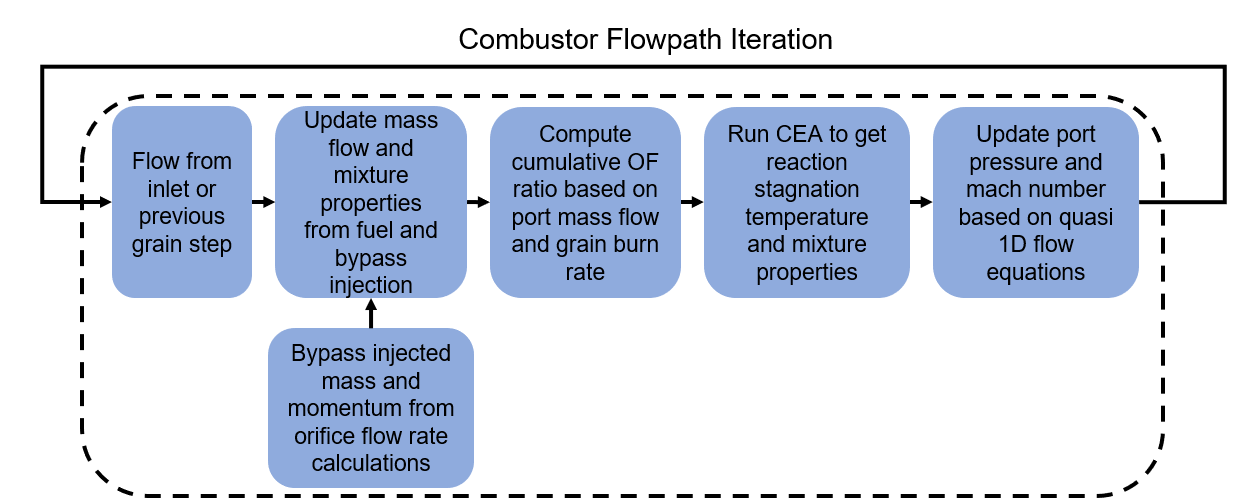
\includegraphics[width=1\textwidth] {Combustor_Figures/flowpath.PNG}
\caption{Combustor Flowpath Loop}
\label{fig:flowpath}
\end{figure}

To begin the flowpath simulation, flow properties are taken as inputs. To fully define the flow, the properties that need to be defined are mass flow rate, temperature, pressure, gamma, Cp, and molecular weight. For the SFRJ simulation, mass flow rate, stagnation temperature and pressure are taken from the output of the inlet object. Molecular properties are taken from air since no chemical reactions are occuring until the combustor is simulated. To iterate along the length of the fuel grain, the combustor port is estimated as a series of discrete control volumes as seen below in Fig. \ref{fig:controlvolume}\\ \indent

\begin{figure}[hbt]
\centering
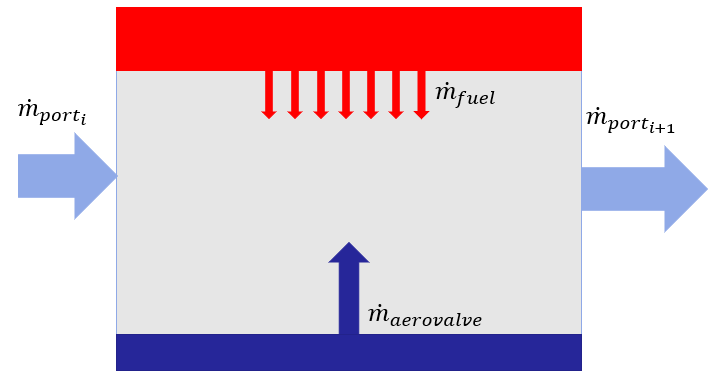
\includegraphics[width=.5\textwidth] {Combustor_Figures/grain_sections.PNG}
\caption{Differential Combustor Port Element}
\label{fig:controlvolume}
\end{figure}

At the beginning of each differential port section, fuel mass flow rate is calculated according to the equation $\dot{m}_f=r_b  \rho  A_b$, where $\dot{m}_f$ is the mass flow of fuel into the port, $r_b$ is the fuel grain burnback rate in meters per second, $\rho$ is the fuel grain density and $A_b$ is the burn area of the fuel grain exposed to the flow. These three fuel grain properties are known inputs in the flowpath loop calculated from the previous time step. Their calculation is discussed in the subsequent sections. At each section of the port there is also the possibility of mass injection of air through the use of the AeroValve component. Flow entering the combustion chamber is diverted to a smaller tube and allowed to pass back into the port through a series of orifices. The mass flow of air entering the combustor is computed using the pressure in the aerovalve along with incompressible orifice flow calculations. With the continuity equations for mass balance satisfied for the discrete grain section, the simulation of combustion can begin. OF is calculated as a cumulative Oxidizer - to - fuel ratio based on the total mass flow in the port to all of fuel that has entered the port. This OF is put into a CEA calculation for estimation of the reactions occuring between the incoming air and the fuel grain. With the implementation of a native CEA runner in MATLAB the computational cost of running  a full chemical simulation is mitigated. The stagnation temperature due to combustion, as well as the new $\gamma$, Cp, and molecular weight due to reactions is taken from the output of the CEA simulation. Using equations derived in \cite{hyball}, conservation of momentum and energy can be applied to the differential port section to iterate to the new mach number and pressure in the port. The equations used for this analysis are shown below.  \\ \indent

\begin{equation}
\centering   
\frac{dM}{M}=F_1 (\frac{dH}{C_pT}+\eta\frac{d\dot{m}}{\dot{m}}-\frac{dMw}{Mw})-.5\frac{d\gamma}{\gamma}
\end{equation}

\begin{equation}
\centering   
\frac{dP}{P}=F_2 (\frac{dMw}{Mw}-\frac{dH}{H}-2\eta\frac{d\dot{m}}{\dot{m}}) 
\end{equation}
where
\begin{equation}
\centering   
\frac{dH}{C_pT}=\frac{d(C_pT_c)-(dC_p)\Bar{T}}{C_pT}
\end{equation}

\begin{equation}
\centering   
F_1=.5\frac{1+\gamma M^2}{1-M^2}
\end{equation}

\begin{equation}
\centering   
F_2=\frac{\gamma M^2}{1-M^2}
\end{equation}

\begin{equation}
\centering   
\eta=1+\frac{\gamma-1}{2}M^2
\end{equation}

With all of these steps we are able to track the pressure, temperature, mach number, and mass flow along the length of the combustion chamber. After the flowpath is simulated the mass flow and port area are known at each discrete location and known. With these variables, the fuel burn rate can be computed for the next time step using the equation $r_b=aG_{Ox}^n$, where a is the burn rate coefficient, .49 mm/s and n is the burn rate exponent, .61. $G_{Ox}$ is the port mass flow per unit area. The regression model and coefficient models are determined experimentally for HTPB in \cite{Pourpoint}. The SFRJ performance sensitivity to inaccuracies in the burn rate coefficients is discussed in a later section. \\ \indent

To simulate the full flight vehicle properly, there must be mass flow continuity through the full flow path of the system from inlet, through the combustor and aerovalve, and through the nozzle. The flow in each of these sections must have cross-talk so that mass flow is conserved properly and flow does not choke or unchoke at the wrong location. The mass flow rate and total temperature entering the vehicle is set by the flight mach number and the inlet capabilities. These are treated as fixed inputs. The pressure at the start of the combustor is an unknown parameter. To ensure proper choking at the nozzle throat after the combustor, an iterative solving loop is implemented. This solving loop pre-populates the combustor flowpath function and solves for the flow along the length of the fuel grain. It then checks if the flow is properly choked at the nozzle throat. If the flow is not choked properly, the pressure guess is changed successively until the throat is choked. This final pressure value is saved and used as the initial pressure guess for the next time step of the simulation. In a physical sense, this pressure solving loop represents the shock train in the inlet needing to respond to the downstream conditions in the combustor to satisfy continuity. If the pressure needed to choke the nozzle throat becomes too high for the inlet to provide, the inlet unstarts and the simulation fails for current design conditions. At the end of the combustion simulation at each time step the fuel burn rate is used to update the fuel grain geometry. With the simple cylindrical grain which was used for much of the simulations performed, an analytic equation for the burn area and port area as a function of grain burnback distance can easily be obtained. For more complex grain shapes such as a finocyl type, a code to generate a table of burn and port areas as a function of burnback is obtained from a custom-developed level-set code which is to be discussed in a later section. A flowchart of the full combustor simulation can be seen below in Fig. \ref{fig:timeloop}  \\ \indent


\begin{figure}[H]
\centering
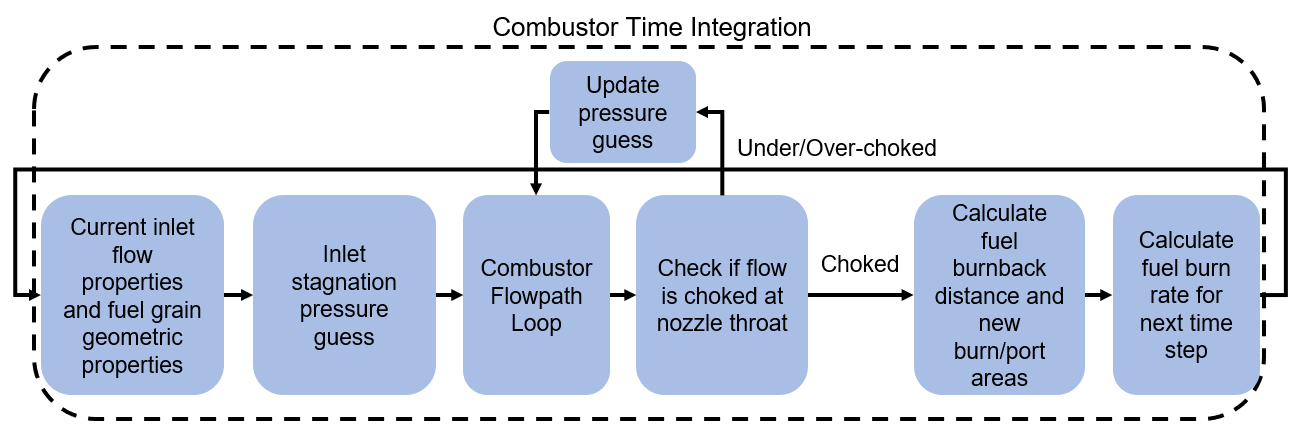
\includegraphics[width=1\textwidth] {Combustor_Figures/timeloop.PNG}
\caption{Iteration of Combustor Properties over Time}
\label{fig:timeloop}
\end{figure}


The flight simulation of the SFRJ is a highly dynamic process, with environment variables such as flight speed, grain geometry, mass flow rate and aerovalve throttling changing constantly throughout the time that the combustor is burning. This can be observed in the plots of operating parameters down the length of the fuel grain at different snapshows during the burn. The first parameter tracked is the oxidizer to fuel ratio seen in Fig. \ref{fig:OF}. In this plot the different flight states can be seen. During the beginning of the burn, the aerovalve allows for air the be injected in the beginning of the fuel grain. This keeps the OF ratio high and allows for flame stabilization on the incoming jet of air. During the middle burn phase two small spikes in the OF ratio can be seen near 5 and 10 inches. This air injection facilitates a higher thrust level so that the vehicle can maintain its flight speed during maneuvers. At the end of the burn the grain begins to burn out from the rear sections.\\ \indent

\begin{figure}[H]
\centering
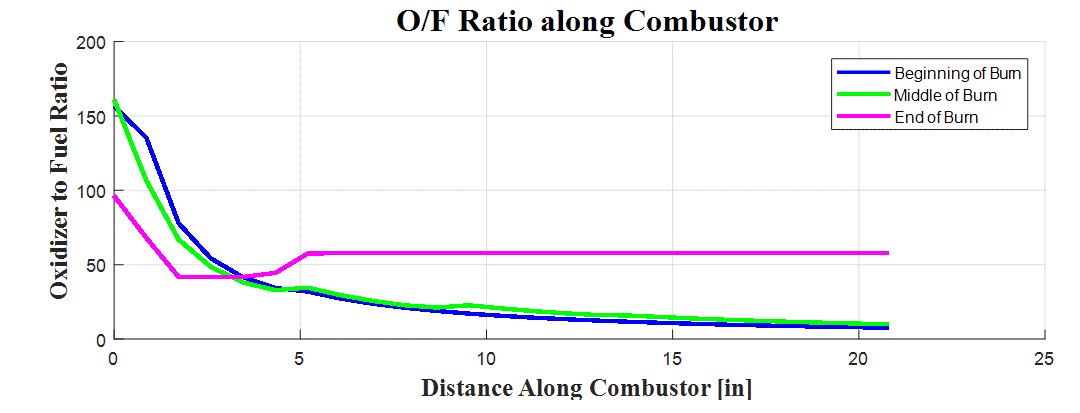
\includegraphics[width=1\textwidth] {Combustor_Figures/OF.png}
\caption{Oxidizer to Fuel Ratio in the Combustor}
\label{fig:OF}
\end{figure}

The same flight states previously described can also be seen well in the port mass flow plots shown in Fig. \ref{fig:massflow}. The large jumps in mass flow in the port can be attributed to discrete air injection locations allowed by the aerovalve to control thrust levels and fuel regression. The mach number plot in Fig. \ref{fig:mach} shows that at the beginning of the burn the mach number in the combustor reaches a maximum slightly above .5. This high speed flow emphasizes the need to take extra care in designing the flameholding sequence near ignition. As the fuel grain regresses the combustor port opens up and the mach number along the fuel grain length decreases significantly. The stagnation temperature and static pressure plots are shown in figures \ref{fig:temperature} and \ref{fig:pressure}, respectively. The maximum value in the temperature plots shows where the combustor is burning the most efficiently. After this point, extending the grain length any longer gives a decrease in efficiency for the system. For this reason it is desired to keep the grain length short enough that there is still enough oxygen left in the port near the aft end of the combustor so that nearly stoichiometric flame temperatures can be maintained.\\ \indent

\begin{figure}[H]
\centering
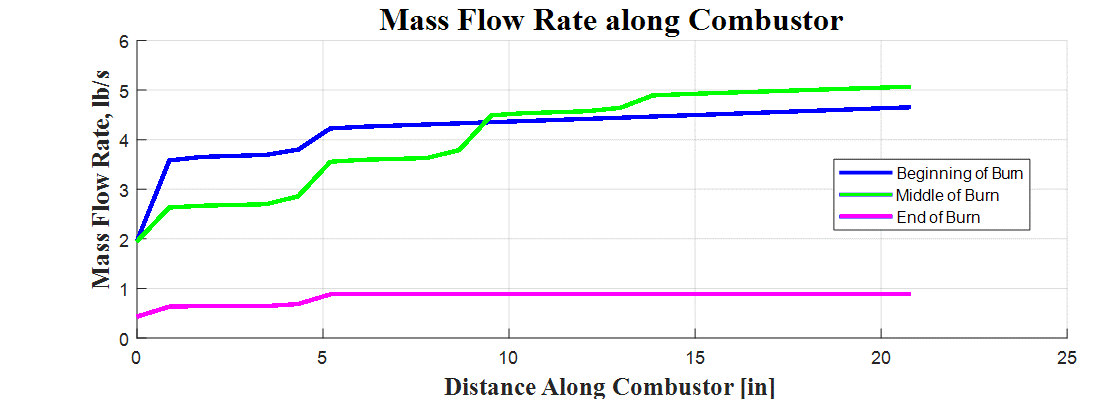
\includegraphics[width=1\textwidth] {Combustor_Figures/Massflow.png}
\caption{Mass Flow Rate in the Combustor}
\label{fig:massflow}
\end{figure}



\begin{figure}[H]
\centering
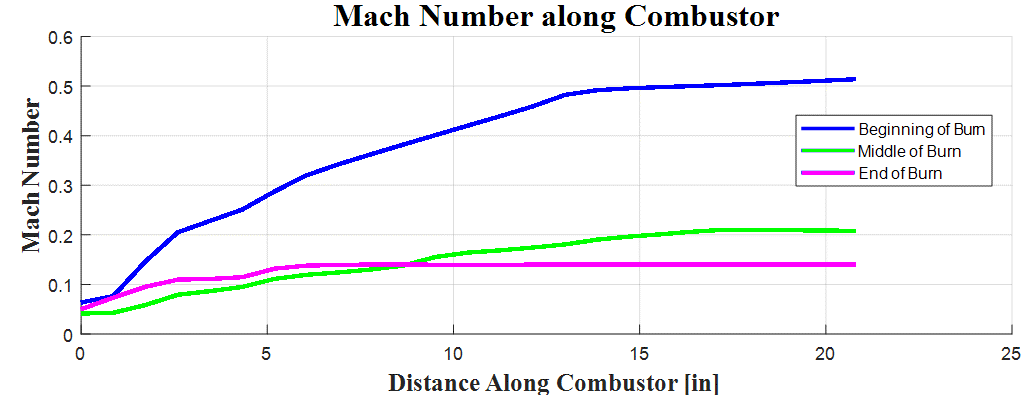
\includegraphics[width=1\textwidth] {Combustor_Figures/Mach.png}
\caption{Mach Number in the Combustor}
\label{fig:mach}
\end{figure}

\begin{figure}[H]
\centering
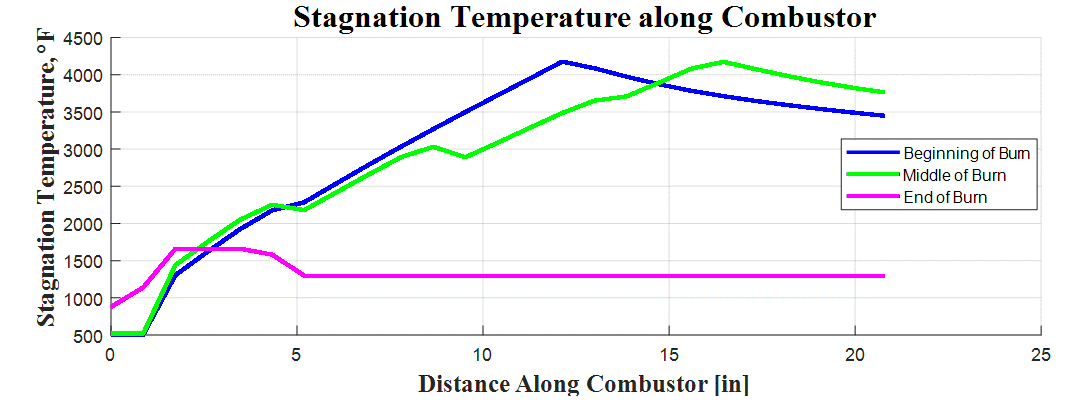
\includegraphics[width=1\textwidth] {Combustor_Figures/Temperature.png}
\caption{Stagnation Temperature in the Combustor}
\label{fig:temperature}
\end{figure}

\begin{figure}[H]
\centering
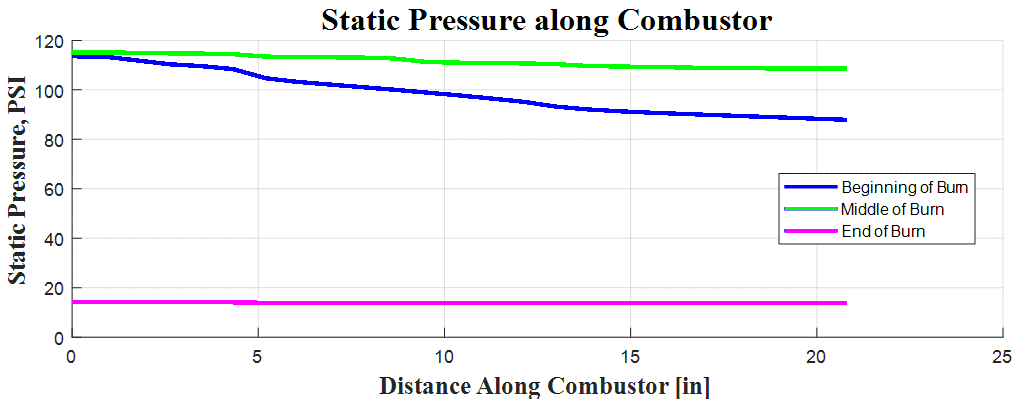
\includegraphics[width=1\textwidth] {Combustor_Figures/Pressure.png}
\caption{Static Pressure in the Combustor}
\label{fig:pressure}
\end{figure}

\subsubsection{Burn Rate Sensitivity Analysis - Jordan Fisher}
As stated previously, the fuel regression rate model was taken from \cite{Pourpoint}. This work presents empirical values for burn rate coefficients for HTPB burning in an oxygen environment in a hybrid rocket system. This application is similar to our SFRJ but cannot be fully trusted. Until experimental verification of the combustor code and burn rate coefficients can be performed, a key risk area of the design is inaccuracy of the burn rate model. A sensitivity analysis of the performance of the system was conducted to gauge the dependency of key flight parameters such as ground range, burn time, average thrust and vehicle flight mach number to the fuel grain burn rate coefficient and exponent. Results can be seen in Fig. \ref{fig:sensitivity}. The burn coefficients a and n were varied $\pm 10\%$ from the values prescribed in \cite{Pourpoint}. For most of the tested range of inputs, a variation of about 25\% can be seen in the ground range and burn time. Average thrust and flight mach number vary by a range of about 10\%. Below the solid black line seen on each plot is a region of unstarted operation. This area poses a greater risk to the performance of the system. Experimental verification of the combustor model will need to be conducted to anchor the flight performance predictions more accurately.  \\ \indent



\begin{figure}[H]
\centering
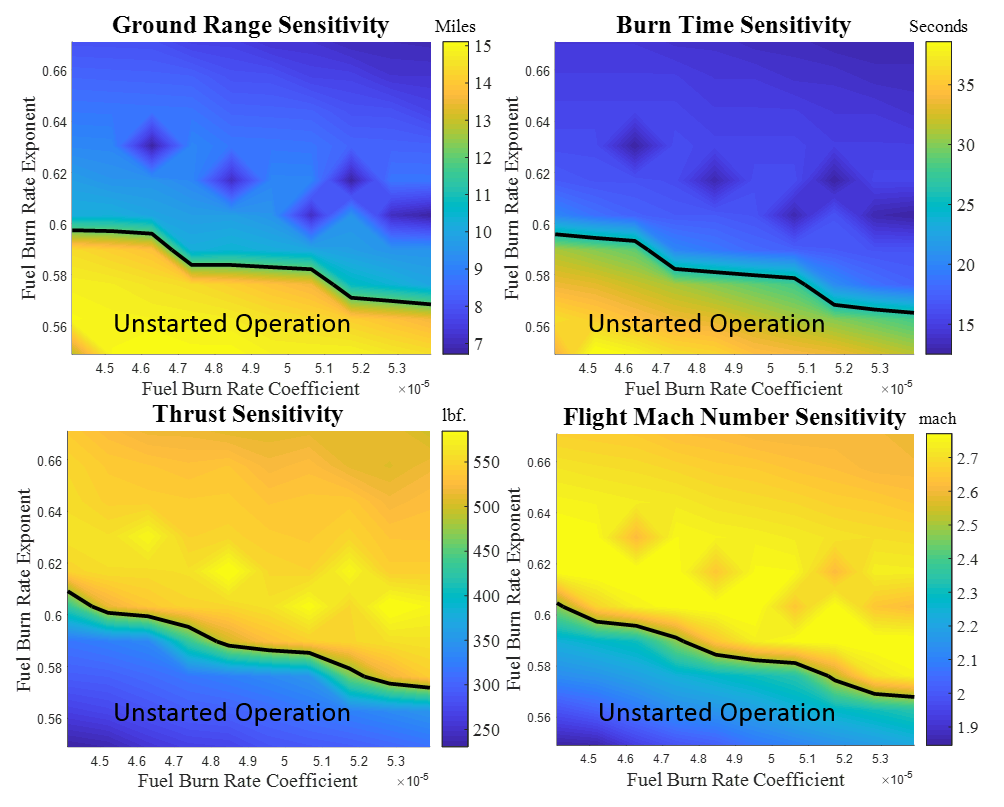
\includegraphics[width=1\textwidth] {Combustor_Figures/sensitivity.PNG}
\caption{Sensitivity Analysis of Various Performance Metrics}
\label{fig:sensitivity}
\end{figure}




